\chapter{第六部分 试题}

%======================================================================
% 力学试题(一)
%======================================================================

\section*{力学试题(一)}

\textbf{1-1}\quad 如力试图1-1所示，轰炸机以速度 $v_{1}$ 作水平匀速飞行，飞行高度为 $H$。

1. 为使炸弹命中地面目标，试问应在离目标多大水平距离处投弹？

2. 在地面上与目标距离为 $D$ 处有一高射炮，在飞机投放炸弹的同时发射炮弹，为使炮弹能击中飞行中的炸弹，试问炮弹初速 $v_{2}$ 至少要多大？

3. 若 $v_{2}$ 取最小值，试问炮弹的发射角是多少？

已知轰炸机、高射炮和目标均在同一竖直平面内。设空气阻力可略。
\vfill

\textbf{1-2}\quad 如力试图2-1，半径为 $R$ 的空心圆环固定在滑块上，滑块放置在光滑水平地面上，滑块与圆环的总质量为 $M$，质量为 $m$ 的小球（看成质点）可在环内作无摩擦运动。开始时小球位于圆环最高点，环与小球均静止。在微小扰动下小球沿环下滑。


1. 试求小球相对地面的轨迹方程。

2. 试用物理方法求小球轨迹（相对地面）在力试图2-1中 $A$、$B$ 两处的曲率半径。

【分析】并入求解之中。
\vfill

\newpage
\textbf{1-3}\quad 如力试图3-1，质量为 $M$、半径为 $R$ 的圆筒垂直放置在光滑水平面上。质量为 $m$ 的小球从圆筒顶部沿圆筒内壁的螺旋构槽无摩擦地下滑。筒高 $h$ 正好等于螺距，即小球沿筒壁绕一周时正好到达筒底。开始时小球与圆筒均静止不动。

1. 试分析下滑过程中圆筒的运动。

2. 试求小球相对地面参考系所走过的路程。
\vfill

\textbf{1-4}\quad 如力试图4-1，质量为 $M$ 的均匀细杆 $AB$ 静止放置在光滑水平面上，$B$ 端的弹簧机构（其质量可略）将质量为 $m$ 的小球（质点）以速度 $v$ 水平弹出，$v$ 的方向与 $AB$ 杆的夹角用 $\varphi$ 表示。要求弹出的小球恰好能与细杆的 $A$ 端相遇（细杆转过的角度不超过 $\pi$）。试确定质量比 $\gamma = \dfrac{M}{m}$ 和角度 $\varphi$ 的取值范围。
\vfill

\newpage
\textbf{1-5}\quad 一陨石在地表上方高为 $h = 4.2 \times 10^{3}\ \mathrm{km}$ 的圆形轨道上绕地球运动，它突然与另一质量小得多的小陨石发生正碰，碰后损失掉 $2\%$ 的动能。假定碰撞不改变大陨石的运动方向和质量。试求大陨石在碰撞后最接近地心的距离。已知地球半径 $R = 6.4 \times 10^{3}\ \mathrm{km}$。
\vfill

\textbf{1-6}\quad 如力试图6-1，质量为 $M$、长为 $2L$ 的均匀细杆用长为 $l$ 的轻绳竖直悬挂起来，保持静止。突然对细杆下端沿水平方向施以短时间的冲量 $J$，绳和细杆均将偏离原来的竖直方向。设绳和细杆偏离竖直方向的角度分别用 $\theta$ 和 $\varphi$ 表示。


1. 试画出运动开始时刻绳与杆的偏离草图。

2. 试问开始时刻绳的角速度 $\dot{\theta}$ 和杆的角速度 $\dot{\varphi}$ 各等于多少？

3. 试问在最大摆角时，$\theta$ 和 $\varphi$ 应有怎样的关系。

\vfill

%======================================================================
% 力学试题(二)
%======================================================================

\section*{力学试题(二)}
\vfill

\newpage
\textbf{2-1}\quad 如力试图1-1，在光滑水平面上有质量为 $M$ 且均匀分布、半径为 $R$ 的圆环。质量为 $m\,(m < M)$ 的质点可在环内壁作无摩擦滑动。开始时，圆环静止，环心在 $O$ 点，质点位于 $(O, R)$ 处，速度沿 $x$ 方向，大小为 $v_{0}$。

1. 试证明质点不会离开环内壁。

2. 试导出质点的运动方程。

3. 试求质点运动轨迹转折处的曲率半径。
\vfill

\textbf{2-2}\quad 如力试图2-1，一宇宙飞船绕地球作圆周运动，圆轨道半径为 $r_{0}$。开动飞船上的喷气发动机可改变运动轨道。假定每次喷气只维持极短的时间，因而喷气时间可忽略；每次喷气后飞船质量可看作不变。喷气后飞船的动量将发生变化，单位质量的动量改变 $\dfrac{\Delta(mv)}{m} = \Delta v$ 称为比冲量。已知地球半径为 $R$，质量为 $M$。


1. 为使飞船从 $r_{0}$ 轨道上逃逸地球的束缚，发动机作第一次喷气。试问所需最小比冲量是多少？

2. 在飞船飞行过程中，飞船作第二次喷气，使它在半径为 $r_{1}$ 的更高的圆轨道上飞行。试问所需比冲量是多少？应向什么方向喷气？

3. 为使飞船从 $r_{1}$ 轨道返回地球，发动机在 $A$ 点作第三次喷气，要求飞船沿地球表面的切向到达 $B$ 点。喷气按两种不同方式进行，一是向正前方，另一是向外侧，试分别计算两种方式所需的比冲量。若 $r_{0} = 2R$，试比较两种比冲量的大小。
\vfill

\newpage
\textbf{2-3}\quad 如力试图3-1，$AB$ 为光滑水平面，$BC$ 是倾角为 $\theta$ 的光滑斜面，两者的连结处 $B$ 可看成是半径为 $r$ 的小圆弧面。质量分布均匀的柔软绳子全长为 $l$，静止放置在 $AB$ 面上，右端与 $B$ 取齐。由于不计摩擦力，只要稍有扰动，绳子将在重力作用下沿斜面下滑。


试求下滑过程中绳子与圆弧边 $B$ 接触处的张力及圆弧边对绳子的支持力，并求绳子脱离圆弧边时绳子的位置。
\vfill

\textbf{2-4}\quad 如力试图4-1，光滑水平桌面上平行放置两匀质长杆 $A$ 和 $B$，长度均为 $l$，质量分别为 $m_{\mathrm{A}}$ 和 $m_{\mathrm{B}}$。杆 $A$ 静止，位于 $x$ 轴上 $(-l + \varepsilon,\, \varepsilon)$ 区域，$\varepsilon$ 是一小量。杆 $B$ 位于 $(0,\, l)$ 区域，并以速度 $v_{0}$ 向 $+y$ 方向作平移运动。当杆 $B$ 运动到 $x$ 轴时，其左端与杆 $A$ 的右端发生完全弹性碰撞。


1. 试求碰后 $A$、$B$ 两杆的质心速度 $v_{\mathrm{A}}$ 和 $v_{\mathrm{B}}$，以及两杆的转动角速度 $\omega_{\mathrm{A}}$ 和 $\omega_{\mathrm{B}}$。

2. 试验证下述公式是否正确：
$$
v_{0} = \left(v_{\mathrm{A}} + \frac{l}{2}\,\omega_{\mathrm{A}}\right) - \left(v_{\mathrm{B}} - \frac{l}{2}\,\omega_{\mathrm{B}}\right)
$$
\vfill

\newpage
\textbf{2-5}\quad 如力试图5-1，质量为 $m$、长度为 $l$ 的两根相同均匀细杆用光滑铰链和一根线连接起来，竖直设置在光滑地平面上，系统原来静止，$\theta_{0} = 30^{\circ}$，突然将线剪断。


1. 试求铰链与平面相碰前的速度。

2. 试求铰链从开始运动到与平面相碰所需的时间（用积分式表示即可）。
\vfill

\textbf{2-6}\quad 如力试图6-1，半径为 $R$、长为 $L$ 的均匀圆柱体，用两根长为 $l$、相距为 $D$ 的平行细线悬挂起来。圆柱体质心 $C$ 的水平位置正好在两悬线之间的正中处。


试求以下三种小振动模式的周期：

1. 两悬线在同一铅垂平面内摆动。

2. 以 $OO'$ 为轴摆动。

3. 绕通过圆柱体质心的铅垂轴摆动。

\vfill

%======================================================================
% 热学试题(一)
%======================================================================

\section*{热学试题(一)}
\vfill

\newpage
\textbf{3-1}\quad 已知 $\nu$ mol 理想气体所经历的某准静态过程中，摩尔热容量 $C$ 可表为
$$
C = \frac{V_{0} - 2\!\left(1 + \dfrac{1}{\gamma}\right)V}{V_{0} - 4V}\,C_{p}
$$
式中 $C_{p}$ 为定压摩尔热容量，$\gamma$ 为绝热指数，$C_{p}$ 和 $\gamma$ 均为常量。设气体体积为 $v_{0}$ 时，其温度为 $T_{0}$。试求气体在该过程中体积从 $v_{0}$ 增为 $2v_{0}$ 的膨胀阶段对外所作的功 $W$。
\vfill

\textbf{3-2}\quad 已知某理想气体的绝热指数 $\gamma$ 为常量，它经历的正循环过程如热试图2-1中实线所示，由两个绝热过程和两个直线过程构成。


1. 已知 $T_{A}$ 和 $T_{B}$，试求循环过程的效率 $\eta$。

2. 设该理想气体为 $1\ \mathrm{mol}$ 的单原子分子理想气体。已知 $T_{B} = T_{0}$，$V_{B} = V_{0}$，$S_{B} = S_{0} = 8R\ln 2$，
$$
T_{A} = 4T_{0},\quad V_{A} = \frac{V_{0}}{8},\quad V_{C} = \frac{V_{0}}{2}.
$$
试求：(a) $T_{C}$、$T_{D}$、$V_{D}$（分别用 $T_{0}$、$V_{0}$ 表示）。(b) $S_{A}$、$S_{C}$、$S_{D}$（均用 $S_{0}$ 表示），并在热试图2-2中画出该循环过程的 $\dfrac{T}{T_{0}} \sim \dfrac{S}{S_{0}}$ 曲线。
\vfill

\newpage
\textbf{3-3}\quad 对流层是贴近地面的一层大气，接近地面的部分在缓慢上升过程中与周围大气的热传递可以忽略。设空气分子中有 $\dfrac{4}{5}$ 的氮分子和 $\dfrac{1}{5}$ 的氧分子。

1. 若地面附近温度为 $27\,^{\circ}\mathrm{C}$，压强为 $1\ \mathrm{atm}$。试求对流层中距地面 $10\ \mathrm{km}$ 高度处的温度。

2. 设在距地面 $10\ \mathrm{km}$ 高度处有一个截面积为 $1\ \mathrm{m}^{2}$ 的球形人造卫星，它以某初速度开始绕地球运动，如果没有大气的阻碍作用，这一初速度恰好能使人造卫星绕地球沿圆轨道运行。然而，由于存在着大气，人造卫星将会受到阻力。为了估算此空气阻力，可将大气分子与卫星的碰撞近似地处理为大气分子与垂直于飞行方向的卫星圆截面之间的弹性碰撞。试估算开始时卫星所受大气阻力的大小。
\vfill

\textbf{3-4}\quad 热容量分别为 $C_{1}$ 和 $C_{2}$ 的两个金属块用一根热容量可忽略不计的粗棍连接起来，整个系统与外界绝热。设 $t = 0$ 时，两金属块的温度分别为 $\tau_{10}$ 和 $\tau_{20}$，设单位时间两金属块之间借助于粗棍传递的热量正比于两金属块的温度差，比例系数 $\kappa$ 为常量。设在此过程中每一金属块内部各处的温度差可以忽略。试求两金属块的温度差降为初始温度差之半所需的时间 $t$，以及在 $t$ 时刻两金属块各自的温度 $\tau_{1}$ 和 $\tau_{2}$。
\vfill

\newpage
\textbf{3-5}\quad 在 NaCl 晶体中，离子间相互作用能量的总和可表为
$$
E_{\mathrm{p}} = N\left(\frac{a_{m}}{r^{m}} - \frac{\alpha e^{2}}{4\pi\varepsilon_{0}\, r}\right)
$$
式中 $N$ 为晶体中正、负离子对的数目，是一个很大的整数，$r$ 为相邻正、负离子的间距，$e$ 为电子电量，$a_{m}$、$\alpha$ 和 $m$ 为常量。$E_{\mathrm{p}}$ 的极小值称为结合能，表为 $E_{\mathrm{p}0}$，相应的相邻正、负离子间距表为 $r_{0}$。任意 $r$ 对应的 $E_{\mathrm{p}}$ 以及 $r_{0}$ 对应的 $E_{\mathrm{p}0}$ 的关系可表为
$$
E_{\mathrm{p}} = E_{\mathrm{p}0} + U
$$
若引入相邻正、负离子间距的相对偏移
$$
x = \frac{\Delta r}{r_{0}} = \frac{r - r_{0}}{r_{0}}
$$
则 $U$ 是 $x$ 的函数。由于 $x$ 一般为小量，可将 $U$ 表为 $x$ 的幂级数，
$$
U(x) = A_{0} + A_{1}\,x + A_{2}\,x^{2} + A_{3}\,x^{3} + A_{4}\,x^{4} + \cdots
$$
通常可近似地只取前几项。如果只取前四项（即取 $U(x) = A_{0} + A_{1}\,x + A_{2}\,x^{2} + A_{3}\,x^{3}$），而且认为相对偏移 $x$ 是由热运动引起的，则由玻尔兹曼统计可以证明（略），当温度为 $T$ 时，$x$ 的统计平均值 $\bar{x}$ 与 $T$ 成正比，即
$$
\bar{x} = CT
$$
其中 $C$ 是表征晶体线膨胀的一个系数，可通过实验测定，亦可表为
$$
C = -\frac{3Nk\,A_{3}}{4A_{2}^{2}}
$$
其中 $k$ 为玻尔兹曼常量。

1. 试导出 $A_{0}$、$A_{1}$、$A_{2}$、$A_{3}$ 各自与参量 $m$、$\alpha$、$r_{0}$ 的关系。

2. 若已测出
$$
r_{0} = 2.81 \times 10^{-10}\ \mathrm{m},\quad C = 7.65 \times 10^{-6}\ \mathrm{K}^{-1}
$$
以及 $r_{0}$ 附近的绝热压缩系数为
$$
\kappa_{s} = -\frac{1}{v}\left(\frac{\mathrm{d}v}{\mathrm{d}p}\right)_{s} = 3.3 \times 10^{-11}\ \mathrm{m}^{2}/\mathrm{N}
$$
试求 $m$、$\alpha$ 和 $a_{m}$ 值。

有用的数学公式：
$$
(1 + x)^{\beta} = 1 + \beta x + \frac{1}{2!}\,\beta(\beta - 1)\,x^{2} + \frac{1}{3!}\,\beta(\beta - 1)(\beta - 2)\,x^{3} + \cdots
$$
其中 $\beta$ 为任意实数。

有关的物理常量：
$$
e = 1.6 \times 10^{-19}\ \mathrm{C},\quad \varepsilon_{0} = 8.9 \times 10^{-12}\ \mathrm{C}^{2}/(\mathrm{N}\cdot\mathrm{m}^{2}),\quad k = 1.38 \times 10^{-23}\ \mathrm{J/K}
$$

\vfill

%======================================================================
% 热学试题(二)
%======================================================================

\section*{热学试题(二)}
\vfill

\textbf{4-1}\quad 已知 $\nu$ mol 的某理想气体在 $T < 2T_{0}$ 时的定体热容量为 $C_{V1} = \alpha \nu R$，在 $T > 2T_{0}$ 时的定体热容量为 $C_{V2} = \beta\, C_{V1}$，其中 $\alpha$ 和 $\beta$ 均为大于 1 的常量。该气体经历的循环过程 ABCDA 是如热试图1-1所示的矩形。


1. 试求状态 D 的温度 $T_{D}$，并画出循环过程中系统内能 $U$ 随温度 $T$ 变化的图线。

2. 试计算循环过程的效率 $\eta$。
\vfill

\newpage
\textbf{4-2}\quad 有两个初始温度分别为 $T_{1}$ 和 $T_{2}\,(T_{2} < T_{1})$ 的大物体，它们的热容量为同一常量 $C$。


1. 用小型热机在这两个大物体之间工作，即从高温大物体吸热向低温大物体放热。由于循环过程中吸热和放热的数量较少，可近似认为两个大物体各自的温度变化只发生在各次循环过程之间，即略去每个循环过程中的温度变化。这样，可将此小型热机设计成可逆卡诺热机，使热机连续工作。试求热机对外作功总量的极限。设整个系统（两个大物体及热机）与外界绝热。

2. 设热机内工作物质为 $\nu$ 摩尔。第一次循环过程的初态温度为 $T_{1}$，工作物质全部为液相，经等压吸热 $L$ 后刚好全部转变成体积为 $V_{1}$ 的气相，尔后再等温膨胀成体积为 $V_{2}$ 的气体，再经绝热等一系列过程后又回到初态。在上述过程中处于气相的工作物质可看作理想气体。试定性画出第一次循环过程中，工作物质一种可能的 $p$--$V$ 曲线和 $T$--$S$ 曲线，并计算热机所作功的大小。
\vfill

\textbf{4-3}\quad 理想气体绝热过程的微观模型。

如热试图3-1，把气体封闭在一柱形绝热气缸内，气缸的一端安置密封无摩擦刚性活塞，将活塞缓慢地向气缸内推进。缸内作热运动的气体分子因与运动的活塞作弹性碰撞而增加动能，增加的动能又通过分子间的相互碰撞为各种形式的内能所均分，结果导致气体温度的相应升高。

试利用此微观模型导出用 $T$--$V$ 关系表述的理想气体绝热过程方程。设绝热指数为常数。
\vfill

\newpage
\textbf{4-4}\quad 如热试图4-1所示，侧面绝热的圆柱形容器被一段长为 $L$ 的圆柱形固态导热均匀介质隔成体积相等的两个区域1和2，其中封有相同分子的理想气体，区域1中气体的质量为区域2中气体质量的两倍。区域1与温度为 $T_{1}$ 的大热源时刻保持热平衡，区域2与温度为 $T_{2}\,(T_{2} > T_{1})$ 的另一大热源时刻保持热平衡。设固态介质不能移动，在长度方向（即圆柱形容器的轴向）有热传导，热传导系数处处相同，在达到稳定的热传导状态时，左端面温度为 $T_{1}$，右端面温度为 $T_{2}$。忽略理想气体内因热传导形成的温度差异，忽略固态介质的热膨胀。


1. 试求固态介质在长度方向上的温度分布。

2. 设区域1气体中的一个分子从 $t = 0$ 时刻出发，经 $t$ 时间后，该分子所处位置与初始位置的间距为 $R_{1}$；同样，设区域2气体中的一个分子从 $t = 0$ 时刻出发，经 $t$ 时间后，该分子所处位置与初始位置的间距为 $R_{2}$。设该分子在 $t$ 时间内未与容器壁碰撞，设 $t$ 远大于分子相邻两次碰撞之间的平均时间。试求 $R_{1}$ 与 $R_{2}$ 的比值。

3. 设理想气体定体摩尔热容量 $C_{V}$ 为常量，设区域2中气体摩尔数为 $\nu_{2}$。设固态介质的摩尔数为 $\nu$，设固态介质的摩尔热容量 $C$ 为常量，且有 $\nu C = 2\nu_{2}C_{V}$。现将两个大热源撤去，整个系统（气体与固态介质）与外界绝热，最后达到自身热平衡。试求最后达到热平衡的温度 $T$。
\vfill

\textbf{4-5}\quad 黑体空腔内的热辐射场可以视为包含各种频率光子的光子气。频率为 $\nu$ 的一个光子的能量为 $h\nu$，质量为 $\dfrac{h\nu}{c^{2}}$。把频率为 $\nu$ 的光子的数密度表为 $n_{\nu}$，则频率为 $\nu$ 的光子的能量密度 $u_{\nu}$ 为
$$
u_{\nu} = n_{\nu}\, h\nu
$$
光子气的总能量密度 $u$ 为
$$
u = \sum_{\nu} u_{\nu}
$$

1. 仿照理想气体的压强，可引入光子气的压强 $p$。

(a) 设空腔的内表面对光子气为完全反射面。试证明，在热平衡时，光子气的压强与能量密度的关系为
$$
p = \frac{1}{3}\,u
$$

(b) 采用热力学第二定律的开尔文表述。试证明 $u$ 与黑体空腔的腔壁材料及空腔体积无关，即 $u$ 仅为温度 $T$ 的函数。进而选取适当的热学公式，证明
$$
u \propto T^{4}
$$

(c) 仿照理想气体准静态绝热过程，可引入光子气的准静态绝热过程。试导出此过程中光子气压强 $p$ 与体积 $V$ 所满足的过程方程。

2. 空腔内光子的运动速率为常量 $c$（真空光速），热平衡时光子在速度方向上的分布具有球对称性。

(a) 光子速度的 $x$ 分量表为 $v_{x}$，一个光子的速度 $x$ 分量处于 $v_{x}$ 到 $(v_{x} + \mathrm{d}v_{x})$ 之间的概率表为 $f(v_{x})\,\mathrm{d}v_{x}$。试证明，
$$
f(v_{x}) = \left\{\begin{array}{ll}
\dfrac{1}{2c}, & -c \leqslant v_{x} \leqslant c \\[6pt]
0, & |v_{x}| > c
\end{array}\right.
$$

(b) 在黑体空腔壁上开一个很小的孔，设不会影响光子气的热平衡。试证明，在单位时间内通过孔的单位截面辐射出去的能量（即能流密度）为
$$
J = \frac{1}{4}\,c\,u
$$
从而有斯特藩--玻尔兹曼定律
$$
J \propto T^{4}
$$

\vfill

%======================================================================
% 电磁学试题(一)
%======================================================================

\section*{电磁学试题(一)}
\vfill

\newpage
\textbf{5-1}\quad 如电试图1-1所示，自由长度为 $L$（足够长），倔强系数为 $k$ 的轻弹簧，两端系两小球1和2。球1的质量为 $m_{1}$，电量为 $Q_{1}\,(Q_{1} > 0)$，球2的质量为 $m_{2}$，电量为 $Q_{2}\,(Q_{2} > 0)$。弹簧与两小球在匀强电场中，场强 $E$ 的方向与球1和球2连线的方向一致。开始时，弹簧为自由长度，两小球静止。设两小球之间的电相互作用以及各种引力均可忽略。


试求尔后两小球之间的最大距离。
\vfill

\textbf{5-2}\quad 如电试图2-1所示，半无限长直载流导线中的电流为 $I$，到达与导线垂直的无穷大平面后，电流均匀地沿垂直平面的径向向四处流去。


试求：1. 右半空间磁场 $B$ 的分布；2. 垂直平面上磁场 $B$ 的分布；3. 左半空间（包括导线所在位置）磁场 $B$ 的分布。
\vfill

\newpage
\textbf{5-3}\quad 质量为 $m$，电量为 $q\,(q > 0)$ 的小球，在离地面高度为 $h$ 处从静止自由落下。为使小球始终不会与地面相碰，可设想在它开始下落时就加上一个足够强的水平匀强磁场。


试求该磁场磁感应强度的最小可取值 $B_{0}$，并画出当磁场取 $B_{0}$ 时小球的运动轨道。设空气阻力可略。
\vfill

\textbf{5-4}\quad 如电试图4-1所示，质量均为 $m$，电量分别为 $q$ 和 $-q\,(q > 0)$ 的两个带电质点相距为 $2R$。开始时，系统的质心 $C$ 静止地位于坐标原点 $O$ 处，且两带电质点在 $xy$ 平面上绕质心 $C$ 沿顺时针方向作圆运动。设当系统处于电试图4-1所示的位置时，规定为 $t = 0$ 时刻，从该时刻起在所讨论的空间范围内加上沿 $z$ 轴方向的弱匀强磁场 $B$。

试求：1. 质心 $C$ 的速度分量 $v_{x}$ 和 $v_{y}$ 随时间 $t$ 的变化关系。

2. 质心 $C$ 的位置 $x$ 和 $y$ 随时间 $t$ 的变化关系。

3. 定性地画出质心 $C$ 的运动轨迹。

设各种万有引力均可忽略。设两质点间的相互作用可近似处理为库仑作用。由于所加磁场很弱，可设两质点相对质心 $C$ 的圆运动近似保持不变。

\vfill

%======================================================================
% 电磁学试题(二)
%======================================================================

\section*{电磁学试题(二)}
\vfill

\newpage
\textbf{6-1}\quad 如电试图1-1所示，电荷线密度为 $\lambda\,(\lambda > 0)$、半径为 $R$ 的均匀带电圆环，固定在光滑的水平绝缘桌面上。质量为 $m$、电量为 $q\,(q > 0)$ 的光滑小球静止地放在桌面上与圆环中心 $O$ 点非常接近的位置处。设圆环上电荷的分布不受小球电荷的影响。


试判断小球尔后的运动是否为振动？若为振动，设小球初始位置与 $O$ 点的距离 $r_{0} \ll R$。试用适当的近似方法，估算小球的振动周期 $T$。
\vfill

\textbf{6-2}\quad 试应用毕奥--萨伐尔定律，求解以下两题。

1. 椭圆形闭合导线的椭圆方程为
$$
\frac{x^{2}}{A^{2}} + \frac{y^{2}}{B^{2}} = 1, \quad A > B
$$
其中 $A$ 和 $B$ 均为已知量。设导线中通以稳恒电流 $I$。试求椭圆焦点处磁感强度 $B_{1}$ 的大小。

2. 在 $x > 0$ 区域有一条无限双曲线形导线，其双曲线方程为
$$
\frac{x^{2}}{A^{2}} - \frac{y^{2}}{B^{2}} = 1
$$
其中 $A$ 和 $B$ 均为已知量。设导线中通以稳恒电流 $I$。试求双曲线内焦点（即在 $x > 0$ 区域中的焦点）处磁感强度 $B_{2}$ 的大小。
\vfill

\newpage
\textbf{6-3}\quad 试讨论带电质点在洛伦兹力的辅助作用下，贴着竖直平面内固定光滑圆环外周作持续圆运动的可能性。

如电试图3-1所示，在竖直平面内有一个半径为 $R$ 的固定光滑绝缘圆环，在空间有垂直环面的水平方向的匀强磁场 $B$。质量为 $m$、电量为 $Q\,(Q > 0)$ 的质点，开始时在圆环最高点 $A$（在圆环外）并具有沿水平方向向左的速度 $v_{0}$。引入两个无量纲的非零正参数 $\lambda$ 和 $\mu$，定义为


$$
\lambda = \frac{v_{0}^{2}}{Rg}, \quad \mu = \frac{Q^{2}B^{2}R}{m^{2}g}
$$
其中 $g$ 是重力加速度。

1. 假设质点能够沿着圆环外周从最高的 $A$ 点到达最低的 $B$ 点，为了使质点而后刚好能够继续作圆周运动而不离开圆环，试问 $\mu$ 与 $\lambda$ 之间应满足什么关系。

2. 对于上述 $\mu \sim \lambda$ 关系，试证明无论 $\lambda$ 取何值（注意 $\lambda > 0$），质点在 $A$ 处必能贴着圆环作圆周运动，且在 $A$ 处质点对圆环的正压力 $N > 0$。

3. 对于上述 $\mu \sim \lambda$ 关系，为使质点在电试图3-1 中 $\pi > \theta > 0^{\circ}$ 位置对圆环的正压力均满足 $N > 0$，即为了使质点必能贴着圆环的左半圆周运动，试求 $\lambda$ 的全部可取值。

4. 对于上述 $\mu$--$\lambda$ 关系，试给出质点必能贴着全部圆环作持续圆周运动的条件。
\vfill

\textbf{6-4}\quad 如电试图4-1所示，平面 $\Sigma_{1}$ 与平面 $\Sigma_{2}$ 相交于直线 $MN$，两平面之间的夹角为 $\phi = 45^{\circ}$，在周围空间有如电试图4-1所示的匀强磁场 $\boldsymbol{B}$，其方向与平面 $\Sigma_{1}$ 平行且与直线 $MN$ 垂直。在平面 $\Sigma_{2}$ 上有一长方形网络，它是由7根长度均为 $l$ 的不同材料电阻丝连接而成的，网络的 $ab$ 边与直线 $MN$ 平行，设各段的电阻依次为 $R_{ab} = R_{fc} = R_{ed} = R$，$R_{af} = R_{bc} = 2R$，$R_{fe} = R_{cd} = 4R$，且电流 $I$ 从 $a$ 点流入，从 $d$ 点流出。


试求电流网络 $abcdef$ 所受磁场安培力的大小 $F$。
\vfill

\newpage
\textbf{6-5}\quad 如电试图5-1所示，半径为 $R$ 的光滑绝缘圆环固定在水平面上，环所在的与水平面垂直的长直圆柱体空间内有均匀磁场，圆柱体空间外无磁场。磁感应强度 $B$ 的基准方向竖直向下。在圆环内有一根质量为 $m$、电量为 $Q\,(Q > 0)$、且都均匀分布的绝缘刚性细杆 $ab$，杆中心与圆环中心的距离为 $\dfrac{R}{2}$，杆两端被约束在环壁上可绕环作无摩擦的运动。设 $t = 0$ 时，杆静止，尔后，因磁场 $B$ 的大小按 $B = B_{0}\sin\omega_{0}t$ 变化，杆在环内先逆时针转过 $2\pi$ 角，再顺时针转回 $2\pi$ 角，并如此不断交替。设杆的运动并不改变杆上电荷的均匀分布。


1. 试确定 $\omega_{0}$ 与 $m$、$Q$、$B_{0}$ 之间的关系。

2. 试确定杆通过其 $a$ 和 $b$ 两端对环所施作用力 $\boldsymbol{N}_{a}$ 和 $\boldsymbol{N}_{b}$ 随时间 $t$ 的变化规律。

\vfill

%======================================================================
% 电磁学试题(三) — 电路
%======================================================================

\section*{电磁学试题(三)}
\vfill

\textbf{7-1}\quad 若二维曲面上分布着稳恒的或似稳的电场 $\boldsymbol{E}$，即若相应的电场线在该曲面上，则曲面上任意两点1和2之间的电势差为
$$
\Delta U = \int_{1}^{2} \boldsymbol{E} \cdot \mathrm{d}\boldsymbol{l}
$$
其中 $\mathrm{d}\boldsymbol{l}$ 是线元矢量，按习惯方式定义。在曲面上引入二维电流密度（实为电流的线密度）$j^{*}$，并引入法向线元矢量 $\mathrm{d}\boldsymbol{l}^{*}$，其大小仍为 $\mathrm{d}l$，其方向与 $\mathrm{d}\boldsymbol{l}$ 垂直，则流过曲面上某段曲线 $l$ 的电流强度为
$$
I = \int_{l} \boldsymbol{j}^{*} \cdot \mathrm{d}\boldsymbol{l}^{*}
$$

1. 设在二维金属曲面上自由电子数的面密度为 $n^{*}$，电子质量为 $m$，电子电量为 $-e$，温度为 $T$ 时自由电子的平均自由程为 $\bar{\lambda}^{*}$，热运动平均速率为 $\bar{v}^{*}$，不考虑磁场力。试导出金属曲面上欧姆定律的微分形式 $j^{*} = \sigma^{*}E$，并给出二维电导率 $\sigma^{*}$ 与 $n^{*}$、$e$、$m$、$\bar{\lambda}^{*}$、$\bar{v}^{*}$ 之间的关系。

2. 在二维曲面上取一段二维流管如电试图1-1所示，端线1和2分别为等势线，因 $j^{*} = \sigma E^{*}$，电试图1-1中带箭头的方向线既表示 $E$ 的电场线又表示 $j^{*}$ 的电流线。若1和2之间的电势差为 $\Delta U$，流过端线1或端线2的电流强度相同，为 $I$，则该段流管的电阻定义为 $R = \dfrac{\Delta U}{I}$。


把二维电阻率（二维电导率的倒数）为常数 $\rho^{*}$ 的金属材料构成如电试图1-2所示的几何面，其侧面是高度为 $H$、半径为 $R_{2}$ 的圆柱面，上、下两端面都是内半径为 $R_{1}$、外半径为 $R_{2}$ 的圆环面。设电流从上端面内圆线均匀流入，从下端面内圆线均匀流出。试求其电阻 $R$。
\vfill

\newpage
\textbf{7-2}\quad 二端电阻网络等效电阻的计算。

1. 在如电试图2-1所示的平面电阻丝网络中，每一直线段和每一圆弧段电阻丝的电阻均为 $r$。试求 $A$ 点和 $B$ 点之间的等效电阻 $R_{AB}$。只要求简单叙述解题步骤，写出必要的中间结果和答案。


2. 如电试图2-2所示的无限内接正方形金属丝网络是由粗细一致、材料相同的金属丝构成的，其中每一个内接正方形的顶点都在外侧正方形四边的中点。已知最外侧大正方形一边的电阻为 $R_{0}$。试求：(a) 网络中 $A$ 点和 $C$ 点之间的等效电阻 $R_{AC}$。(b) 网络中 $E$ 点和 $G$ 点之间的等效电阻 $R_{EG}$。
\vfill

\textbf{7-3}\quad 如电试图3-1所示的电路已经达到稳定状态，两个无内阻电源电动势的正方向分别如电试图3-1中箭头所示，其值为


$$
\mathcal{E}_{1} = \mathcal{E}_{0}\sin^{2}\omega t,\qquad \mathcal{E}_{2} = \mathcal{E}_{0}\cos\omega t
$$

电试图3-1中其他参量为 $R_{1} = R_{2} = R$，$L = \dfrac{R}{2\omega}$，$C = \dfrac{1}{2\omega R}$。设流过电阻 $R_{1}$ 的电流 $i_{1}$ 的正方向如电试图3-1所示。试求 $i_{1}$ 与 $t$ 的关系，并以 $\omega t$ 为横坐标、$i_{1}$ 为纵坐标，画出 $i_{1} \sim t$ 曲线。
\vfill

\newpage
\textbf{7-4}\quad 几何图形化的 $R$、$L$ 网络如电试图4-1所示，其中每一根直线段都代表一条相同的 $R$、$L$ 串联电路，对于所取的交流角频率 $\omega$，有 $\omega L = \sqrt{3}\,R$。


1. 试计算 $A$、$B$ 之间的等效电抗 $Z_{AB}$（复阻抗 $Z_{AB}$ 的模量），答案仅用 $R$ 表示。

2. 以 $A$ 为输入端，$D$ 为输出端，为使 $A$、$D$ 之间网络总功率的功率因素成为 $\cos\phi = \dfrac{\sqrt{2}}{2}$，可在每一支路上串联一个相同的电容 $C_{1}$。试求最小的 $C_{1}$ 值，答案仅用 $\omega$ 和 $R$ 表述。

3. 每一支路都不串联电容，但在 $D$ 点之外串联一个电容 $C_{2}$，使网络 $AD$ 与 $C_{2}$ 构成的串联组总功率的功率因数成为 $\cos\phi = \dfrac{\sqrt{2}}{2}$。试求最小的 $C_{2}$ 值，答案仍用 $\omega$ 和 $R$ 表述。
\vfill

\textbf{7-5}\quad 锯齿波形电源对应的 RC 串联暂态过程。

电路如电试图5-1所示，开始时断路，电容器上无电量。$t = 0$ 时合上电键 $K$，设 $\varepsilon \sim t$ 的关系如电试图5-2所示，且 $T = RC$。


试求 $t = NT\,(N = 1, 2, 3, \cdots)$ 时，电容器正极板上的电量 $Q_{N}$，并给出 $N \to \infty$ 的 $Q_{N}$ 极限。

\vfill

%======================================================================
% 电磁学试题(四) — 电路
%======================================================================

\section*{电磁学试题(四)}
\vfill

\newpage
\textbf{8-1}\quad 截面积为 $S$、长为 $L$ 的圆柱形电阻器如电试图1-1所示，电流从 $x = 0$ 端面均匀地流入，从 $x = L$ 端面均匀地流出。设电阻器的电阻率分布为


$$
\rho = \rho_{0}\left|\sin 2\pi\frac{x}{L}\right|
$$
设电阻器两端面之间所加电压为 $U$。

试求：1. 电阻器的电阻 $R$。

2. 电阻器中体电荷密度 $\rho_{e}$ 的分布及 $\rho_{e} > 0$ 的区域。（体电荷密度 $\rho_{e}$ 与电阻率 $\rho$ 请勿混淆。）

3. 电阻器中 $x = \dfrac{L}{2}$ 处的面电荷密度 $\sigma_{e}$。
\vfill

\textbf{8-2}\quad 内部连通、有 $N$ 个外接端的电阻网络称为 $N$ 端网络。把没有内节点、每两个外接点之间有一个电阻的 $N$ 端网络，称为 $N$ 端标准网络或 $N$ 端完全网络。把有内节点的 $N$ 端网络称为 $N$ 端非完全网络。

可以证明，任何一个 $N$ 端非完全网络，无论所包含的内节点是有限的还是无限的，均可等效变换成一个相应的 $N$ 端完全网络。

1. 试画出四端完全网络。试画出一个由8个电阻（其间并无串并联关系）组成的、含有一个内节点的四端非完全网络。

2. 用电阻丝连成的三端非完全网络如电试图2-1所示，其中每一小段电阻丝的电阻均为 $R$，$A$、$B$、$C$ 是三个外接点。试把这个三端非完全网络等效变换为三端完全网络，并求出后者的各电阻。


3. 用单位长度电阻为 $r$ 的电阻丝连成的网络如电试图2-2所示，其中两个大三角形的边长均为 $a$，从左侧大三角形三边中点开始无限内接小三角形。试求 $A$ 点和 $B$ 点之间的等效电阻 $R_{AB}$。
\vfill

\newpage
\textbf{8-3}\quad 交流电路如电试图3-1所示。


1. 设电源电动势为
$$
\mathcal{E} = \mathcal{E}_{0}\sin^{2}\omega t
$$
且
$$
\omega L = \frac{1}{\omega C} = R
$$
试用矢量图解法求 $i(t)$。

2. 设电源电动势可普遍地表为
$$
\mathcal{E} = \mathcal{E}_{0} + \sum_{i} \mathcal{E}_{io}\cos(\omega_{i}t + \phi_{i})
$$
其中 $\mathcal{E}_{0}$、$\mathcal{E}_{io}$、$\omega_{i}$、$\phi_{i}$ 均为常量，且
$$
R = \sqrt{\frac{L}{C}}
$$
试用复数法求 $i(t)$。
\vfill

\textbf{8-4}\quad 交流电路二端网络如电试图4-1所示，设交流电角频率为 $\omega$。


试求 $A$ 和 $B$ 两端之间的等效复阻抗 $\tilde{Z}_{AB}$。再设 $\omega L = \dfrac{1}{\omega C} = R$。试求 $Z_{AB}$（用 $R$ 表示）及此二端网络的功率因素 $\cos\phi$。
\vfill

\newpage
\textbf{8-5}\quad 长方体导体块如电试图5-1所示，从 $t = 0$ 开始，外加与导体左右侧面垂直的交变匀强电场 $E = E_{0}\cos\omega t$，其中常矢量 $E_{0}$ 的方向已在电试图5-1 中标明。设导体的电导率


$$
\sigma = \alpha\varepsilon_{0}\omega
$$
其中 $\alpha$ 是无量纲的常量。忽略边缘效应（即在需要时可把导体块的侧面视为无穷大平面）。

1. 以 $E_{0}$ 的方向为基准方向，引入导体块中的电流密度 $j$，试求 $t > 0$ 的 $j(t)$ 关系。

2. 导体块左右侧面的大小实际上是有限的，导体块中的电流强度 $i$ 也是有限的。把外电场 $\boldsymbol{E}$ 从导体块左侧面到右侧面的电势降表为 $u$。试求电流达到稳定后，$i$ 超前 $u$ 的相位 $\phi$（用 $\tan\phi$ 表示）。

3. 设导体块左、右侧面的面积均为 $S$，其间的间距为 $l$。另取如电试图5-2所示的并联电路，若当外加电压为第2问中的 $u$ 时，电试图5-2 电路中的总电流刚好是第2问中的 $i$。试求电试图5-2 电路中的 $R$ 和 $C$，又，若电试图5-2 电路中的电容器是平行板介质电容器，极板面积也为 $S$，两板间距（亦即其中介质的厚度）也为 $l$。试求该介质的相对介电常量 $\varepsilon_{r}$，并判断该电容器能否制作。

\vfill

%======================================================================
% 光学试题
%======================================================================

\section*{光学试题}
\vfill

\textbf{9-1}\quad 如光试图1-1所示，物点 $Q$ 位于某凹面反射镜的主光轴上，$Q$ 点与顶点 $O$ 的距离为 $s$。要求从 $Q$ 点发出的所有光线经反射后都能会聚在主光轴上的 $Q'$ 点，$Q'$ 点与顶点 $O$ 的距离为 $s'$。

\begin{center}[htbp]
\centering
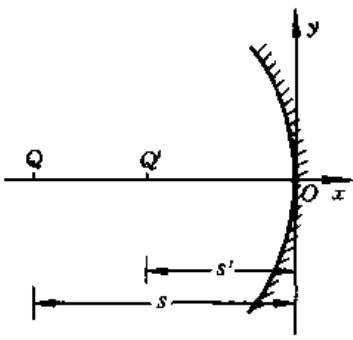
\includegraphics[width=0.6\textwidth]{figures/光试图1-1.jpg}
\end{center}

试根据费马原理证明凹面是一个旋转椭球面，即曲面与 $xy$ 平面的截线是一个椭圆，写出椭圆的方程式，并求椭圆中心的位置和长、短半轴。
\vfill

\newpage
\textbf{9-2}\quad 在如光试图2-1所示的薄透镜系统中，透镜 $L_{1}$ 和 $L_{2}$ 的焦距 $f_{1} = f_{2} = 10\ \mathrm{cm}$，两透镜的间距为 $70\ \mathrm{cm}$，物在 $L_{1}$ 前方 $20\ \mathrm{cm}$ 处。

\begin{center}[htbp]
\centering
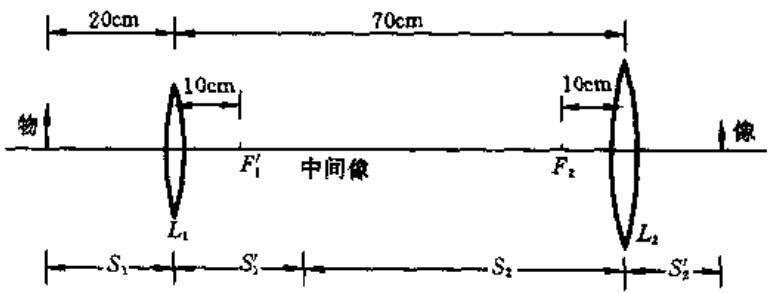
\includegraphics[width=0.6\textwidth]{figures/光试图2-1.jpg}
\end{center}

1. 试求最后像的位置、大小和正倒。

2. 为提高光能利用率（增加系统的聚光能力），可增加第三个会聚透镜 $L_{3}$，为了使最后像的位置仍保持不变，试问 $L_{3}$ 应放在何处？

3. 试借助于特殊光线用作图法解释 $L_{3}$ 能提高聚光能力的原因。
\vfill
